\section{Slow Cycle: Social Network Model}\label{sec:slowCycle}


This section will first introduce the basic framework of Social Network Model and how it is integrated into the TDR system. And then describe the two track of the Social Network Modeling: (1) how to upload the judgements to the database and (2) how to update the weight of each profile in the model.

\subsection{Social Network Model Framework}


\begin{figure}[ht]
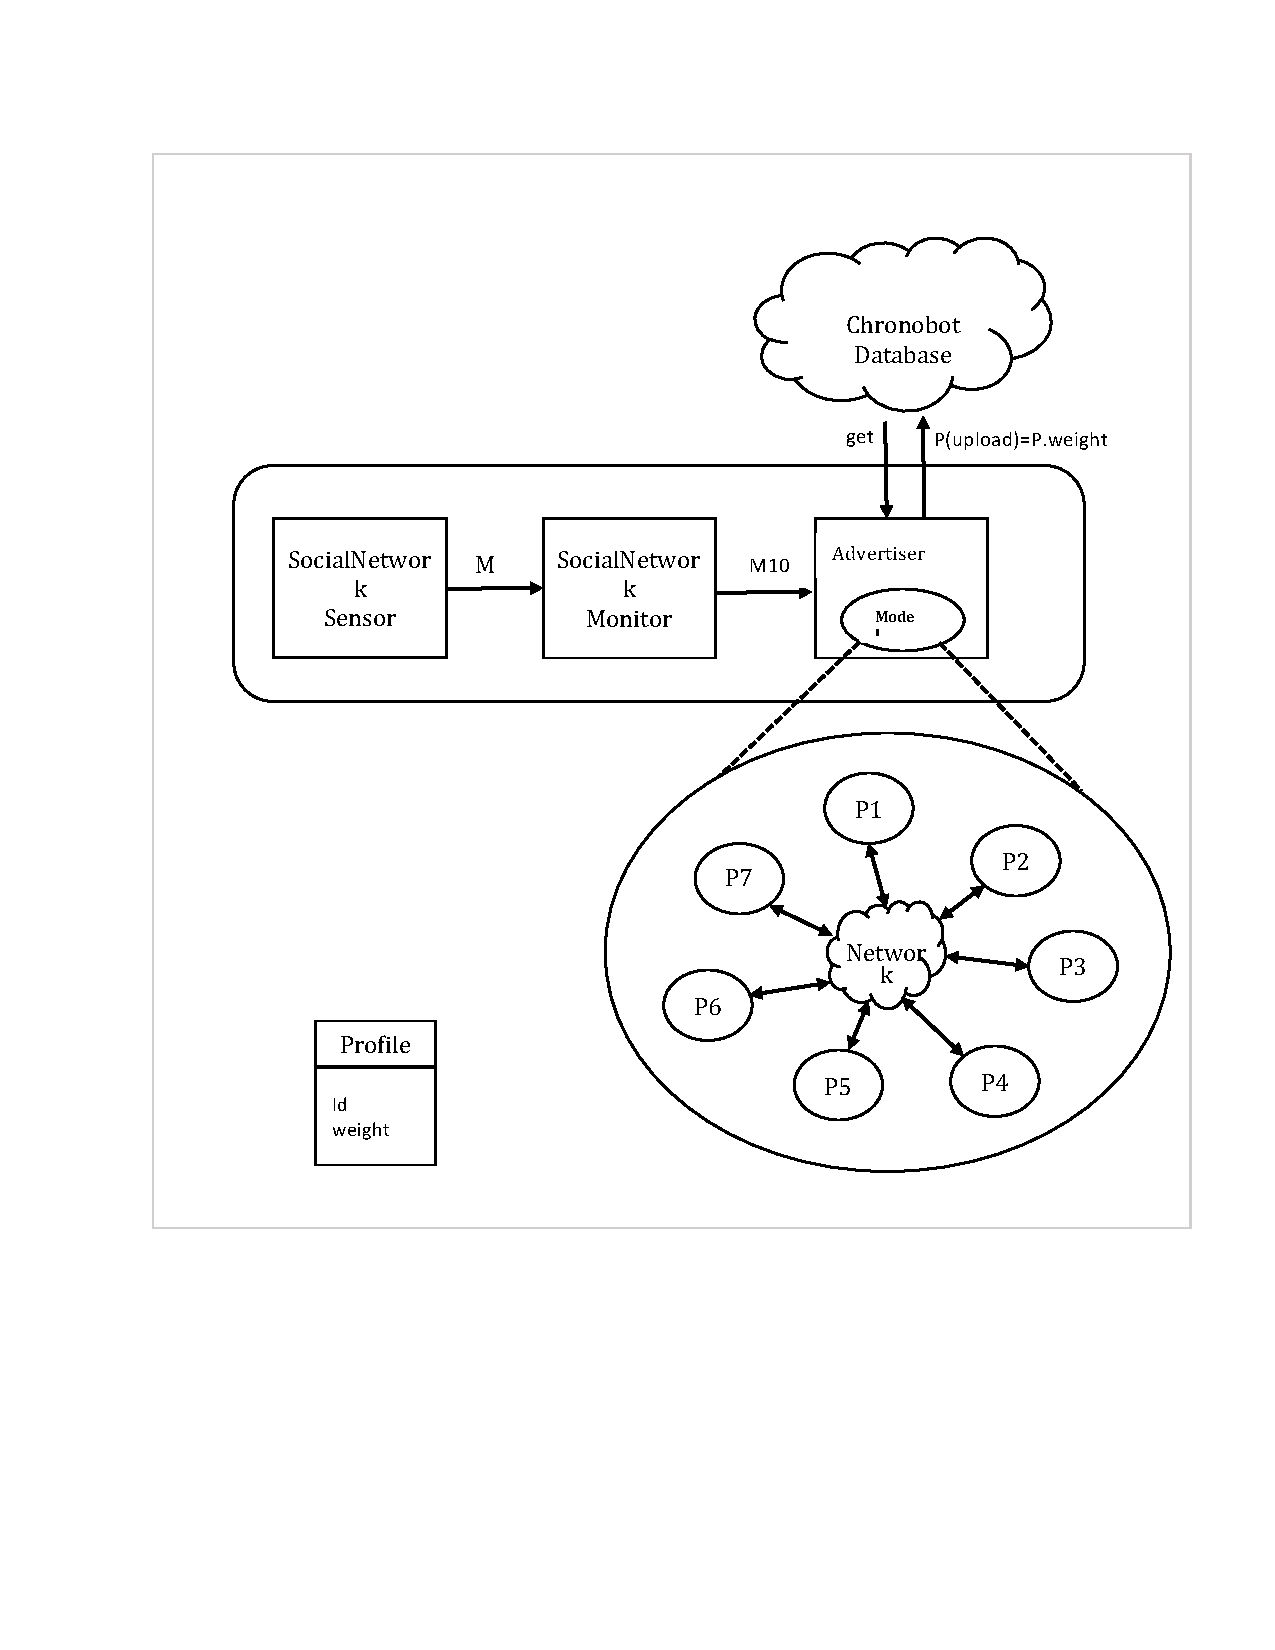
\includegraphics[width=0.9\columnwidth]{socialnetwork/SocialNetworkModel}
\caption{SocialNework Framework}
\label{fig:outliner}
\end{figure}


\subsection{Teacher-Student Model}
 A profile in the group with higher weight is more reliable in judging others and we call this kind of profile teacher profiles. In the group model, there is one or more profile which is called teacher profile who has a higher weight while the other profiles own lower weights. The basic mode for each profile are two attributes: a $profile_id$ which can uniquely identify the profile in the model and a $profile_weight$ which represents the reliability of the judgements generate by the profile.
 
 \subsubsection{Judgement Upload Track}
 Judgements from different profile int the model are not treated equal in our model. A teacher profile may always make judgements corresponding with the real status of the target. In other words, a teacher is more likely to generate the correct judgements in the model. Thus we should accept all the judgements from the teacher and treat them as Oracle who always knows the truth. Accordingly, the weight of a teacher is set to be 1. On the other hand, the tiro-students who don't know how to make Chi judgements are less likely to generate reliable judgements and thus their judgements are not accepted by the system. In fact, there are intermediate students whose judgement ability is between a tiro-student and the teacher and there must be a threshold $\theta$ where the weights large than it are treated as teacher-like weights. Thus we should find out where the $\theta$ stays and distinguish the teacher-like students and accept their judgements. As time goes by, students are going to behave like teacher and generate reliable judgements.
 

  \subsubsection{Judgement Upload Track}
 The weight of a profile is related to the average distance of judgements with the teacher profile in history. For each time point $n$ where the computation cycle happens, the weight of a $profile_i$ can be updated by the following equation.
\begin{equation}
  W_i= \dfrac{\sum_{t=1}^{n} dist( J_it - J_ot )}{n}
\end{equation},
where $J_it$ is the judgement at time t by $profile_i$ and $J_ot$ is the judgement by the teacher at time t. The $W_i$ considers all the history distance of a specific profile to the teacher. If a student knows nothing about making Chi judgement at first and finally grasp the method, and his judgments will be accepted after a time point $t$. 